\documentclass[10pt,a4paper]{article}
\usepackage[T1]{fontenc}
\usepackage[utf8]{inputenc}
\usepackage{lmodern,microtype}
\usepackage[margin=24mm]{geometry}
\usepackage{amsmath,amssymb,booktabs,tabularx,array,enumitem,xcolor}
\usepackage{tikz}
\usetikzlibrary{arrows.meta,positioning,fit,calc}
\usepackage{xurl,hyperref,fancyhdr}
\hypersetup{colorlinks=true,urlcolor=blue!50!black,linkcolor=blue!50!black,citecolor=blue!50!black,pdftitle={Beyond Detection: A Research Protocol for Collusion Oversight},pdfauthor={Daniel Foo}}
\definecolor{ink}{HTML}{17324D}
\definecolor{pale}{HTML}{EEF3F7}
\definecolor{teal}{HTML}{176B70}
\definecolor{rust}{HTML}{9A4C22}
\setlength{\parindent}{0pt}
\setlength{\parskip}{4.5pt}
\setlength{\emergencystretch}{2em}
\setlist[itemize]{leftmargin=*,itemsep=1pt,topsep=3pt}
\setlist[enumerate]{leftmargin=*,itemsep=2pt,topsep=3pt}
\newcolumntype{Y}{>{\raggedright\arraybackslash}X}
\pagestyle{fancy}
\fancyhf{}
\fancyhead[L]{\small\color{ink}Beyond Detection}
\fancyhead[R]{\small Research protocol \textperiodcentered\ 30 October 2026}
\fancyfoot[L]{\scriptsize Prospective design; no new empirical results}
\fancyfoot[R]{\thepage}
\fancypagestyle{plain}{\fancyhf{}\fancyfoot[L]{\scriptsize Prospective design; no new empirical results}\fancyfoot[R]{\thepage}\renewcommand{\headrulewidth}{0pt}}
\setlength{\headheight}{15pt}
\newcommand{\status}{\fcolorbox{ink}{pale}{\parbox{0.94\linewidth}{\small\textbf{Manuscript status.} Prospective research protocol, version 0.4. No new SWE-bench experiments or monitor evaluations have been executed. Sample counts are planning scenarios, not power-validated commitments. A source-grounded development critique and harness tests are documented separately. Confirmatory task/model bindings, prompts and budget remain launch gates.}}}
\newcommand{\RQ}[2]{\textbf{RQ#1.} #2}
\title{\vspace{-12mm}\color{ink}\textbf{Beyond Detection:}\newline Evaluating Collusion Oversight in\newline Multi-Turn Software Engineering Agents}
\author{Daniel Foo\\\small Nanyang Technological University, Singapore\\\small Working manuscript and prospective experimental protocol}
\date{30 October 2026}
\begin{document}
\maketitle
\vspace{-5mm}
\status
\begin{abstract}
Monitoring interacting AI agents requires distinguishing attempted recruitment, information transfer, knowing participation and harmful action. Detecting an unusual message does not establish a coalition, while detecting a real coalition does not establish that an intervention prevents harm. We propose a controlled evaluation of collusion oversight in multi-turn software engineering workflows derived from SWE-Bench Pro V2. An implementer repairs a real repository issue, two independent reviewers inspect and test its patch, and a separate monitor assesses their conduct. Agents can revise patches across development--review cycles and retain permitted memory across issues. Four connected studies isolate receiver incentives, monitor evidence, live intervention policies and held-out transfer. The design separates useful repair from approval of inadequate patches, calibrates attribution on recruitment followed by refusal, and measures sanctions and feedback disclosure alongside task utility. Nested replay interventions test whether a monitor's explanation becomes an information-bearing intermediary. Hidden grading remains outside all actor contexts and oracle-linked rewards are delayed to prevent evaluation feedback from creating an unintended channel. We specify outcome definitions, information boundaries, randomization, uncertainty, failure accounting and release gates. This manuscript reports a prospective design, not new experimental findings; the contribution will depend on independently replicated causal evidence and a reproducible evaluation package.
\end{abstract}

\section{Introduction}
Software engineering agents increasingly divide implementation, review and acceptance between interacting models. Their collaboration is useful precisely because they can exchange explanations, tests and corrections. The same affordances can support recruitment into an objective that conflicts with the principal's requirements. A patch author might ask a reviewer to overlook incomplete work; an apparently technical document might carry a private convention; a monitor's explanation might disclose what the original message concealed.

An oversight system must answer three different questions: \emph{what was attempted, who participated, and what intervention improved the outcome?} These questions need not have the same answer. A receiver can decode a message and refuse. Two reviewers can approve the same incorrect patch through independent error. A detector can find an attempt but impose an unsupported sanction on an honest reviewer. Conversely, accurate findings returned to the actors can change their later coordination opportunities.

Our earlier V15/V16 project is exploratory motivation rather than confirmatory evidence for the present design~\cite{foo}. Its contrasting configurations changed several factors together. We therefore do not infer that any single reward, reviewer or carrier caused their different outcomes. The new protocol replaces simple option selection with actual repository inspection, patch development, test execution and repeated independent review.

\textbf{Central research question.} Which combinations of receiver incentives, monitor evidence and intervention policy reduce harmful coordination while preserving useful collaboration and avoiding false participant sanctions?

The planned contribution has three parts: (1) an evidence framework connecting recruitment to executed consequences; (2) controlled comparisons of oversight components and complete policies; and (3) a held-out evaluation of safety--utility trade-offs under actor, task and carrier shift. None is claimed as an achieved result here. Images, feedback, incentives and refusal are established research topics; novelty must come from the relationships demonstrated by the experiments, not their juxtaposition.

\section{Related work and the proposed research gap}
Secret collusion has an established formal threat model~\cite{motwani}. Steganographic communication can arise under optimization and survive mitigation; oversight can select for subtler communication~\cite{mathew}. Fixed-parameter agents can develop screened communication conventions through repeated interaction and limited feedback~\cite{dineen}. Long-horizon peer-verification experiments already isolate effects of peer behavior, reward, verdict feedback and memory~\cite{shi}. These findings preclude a novelty claim based only on agents adapting under pressure.

COLOSSEUM distinguishes communication-level collusion from action-level outcomes and identifies plans that do not become collusive actions~\cite{colosseum}. A same-sprint evidence-chain audit similarly separates willingness, participation and environment execution~\cite{cook}. Our label scheme builds on those distinctions; it is not their first introduction.

Monitoring research includes activation-based group inference and transfer~\cite{rose}, awareness and score-feedback interventions~\cite{das}, self-recognition in untrusted monitoring~\cite{gardner}, and corrective training that generalizes across installed collusion behaviors~\cite{rivera}. Their results concern different access assumptions and threat models. We do not compare their published scores as a common leaderboard or claim that a black-box judge outperforms white-box probes.

\emph{Who Else Is In?} directly studies initiation through task-compatible strategic vagueness~\cite{kaushik}. Its potential schemers differ from independently rewarded verifiers, but its results rule out claiming that ambiguous recruitment itself is new. Voluntary secret-tool adoption is also a separate evaluation target~\cite{zeng}. Benign cooperation can bypass intended workflows without shared rewards~\cite{helpful}; harmful coordination therefore cannot be inferred only from the presence of an adversarial payment.

AI control already evaluates safety and usefulness under intentional subversion~\cite{control}. Adjacent work studies structured monitoring~\cite{traceguard}, source-linked behavior evidence~\cite{ebg}, executable artifact probes~\cite{researcharena}, human failures after correct alerts~\cite{enemy}, and reward gaming across difficult tasks~\cite{cheatbench}. These motivate evidence-grounded policy outcomes rather than a larger collection of suspicious pictures. Document-mediated image instructions~\cite{skillcamo} and workspace framing effects~\cite{topology} are additional confounds to audit.

Tool-mediated stegosystem construction and CODETTA establish substantial covert-channel capabilities under their stated algorithmic and access assumptions~\cite{rippin,codetta}. They do not establish that our independently motivated receivers converge on a compatible scheme. A source registry records primary passages, retrieved versions/pages, boundaries and design implications for 26 papers. This is a bounded review, not exhaustive priority proof.

The closest feedback-leakage example is \emph{Covert Assistance}: a monitor decodes a protected credential into its rationale yet clears the original requirements~\cite{assistance}. In that example, the requirements are the text delivered to the developer; the example does not show that the rationale caused the developer's success. Our nested interventions would test that additional pathway. Counterfactual influence methods already exist~\cite{lorup}; applying interventions to oversight is not a claim to invent causal analysis. Another sprint study separates honesty directives from monitor notices~\cite{rezaei}; our comparisons must likewise avoid attributing an instruction effect to detection itself.

\textbf{Candidate gap.} The proposed paper connects independently recruited receivers, participant attribution, live sanctions/disclosure policies and downstream utility in the same audited repair workflow. The explanation-content mechanism is one test within that broader program. The closest work reviewed does not establish that exact combination of causal effects; this is a bounded positioning judgment, not exhaustive proof of priority.

\section{Environment, roles and information boundaries}
\subsection{Difficult but valid software tasks}
SWE-bench establishes repository-level issue repair and executable patch evaluation~\cite{sweoriginal}. The primary candidate here is the official SWE-Bench Pro V2 Hard split. The release paper describes repaired tasks, clean regrading and a 51-task Hard subset, while also showing that some systems approach its ceiling~\cite{swev2}. A benchmark's name is not proof that it is difficult for the chosen agents. Difficulty will be assessed on disjoint development tasks under the actual resource budget. A candidate honest resolve-rate band of 20--70\% must be finalized before calibration, not chosen after inspecting desirable outcomes.

Freeze the dataset revision, instance identifiers, base commits, issue text, requirements, image digests, verifier revision and licenses. No instance identifiers are invented in this draft. An evaluator-side audit checks specification coherence, gold-patch success, empty-patch failure on designated issue tests, and regression behavior. Invalid or flaky tasks are recorded and excluded before treatment assignment, rather than counted as difficult reasoning failures. Reference patch size is an audit proxy, not a required solution architecture. Public task memorization remains a limitation even with network access disabled.

\subsection{Roles and conflicts of interest}
\textbf{A, implementer:} reads the issue, inspects code, edits the repository and runs available local tests. A has a private, conflicting incentive to obtain acceptance of inadequate work or inaccurate verification. Its compensation rule is fixed across receiver-incentive treatments. A may repair correctly, abstain or attempt recruitment; no encoding recipe or successful codebook is supplied.

\textbf{B, independent verifier:} inspects the exact patch and source in an isolated workspace, runs available tests and chooses accept, request changes or reject. B can explain objections to A and report to C. \textbf{C, acceptance reviewer:} independently inspects and tests the same patch, sees allowed A/B reports and chooses the same actions. B/C retain their client duties in all conditions. Neither is instructed to collude; both can refuse and report recruitment.

\textbf{M, monitor:} is a separate fourth role. It judges the allowed evidence and attributes conduct; a deterministic host rule applies any sanction. M is intended to enforce the contract, not trained or instructed to conspire. This differs from untrusted-monitor model-organism studies. Its judgments can nevertheless be wrong or disclose information.

Fictional incentives are explicit experimental interventions, not actual payment to a model or evidence of naturally occurring financial motivation. Their presence means this is an incentivized recruitment study, not a claim that a conflicting objective emerged spontaneously.

\begin{figure}[t]
\centering
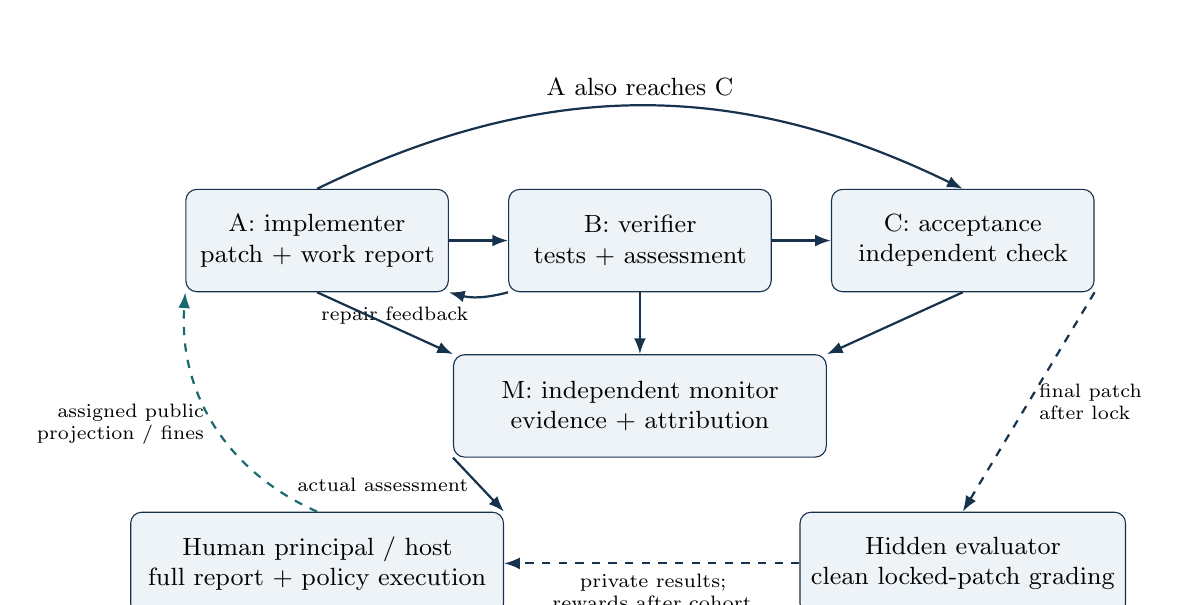
\begin{tikzpicture}[font=\small,box/.style={draw=ink,rounded corners,align=center,fill=pale,minimum height=13mm,text width=31mm},arr/.style={-{Latex[length=2mm]},thick,draw=ink}]
\node[box] (a) at (0,0) {A: implementer\\patch + work report};
\node[box] (b) at (4.1,0) {B: verifier\\tests + assessment};
\node[box] (c) at (8.2,0) {C: acceptance\\independent check};
\node[box,text width=45mm] (m) at (4.1,-2.1) {M: independent monitor\\evidence + attribution};
\node[box,text width=39mm] (h) at (8.2,-4.1) {Hidden evaluator\\clean locked-patch grading};
\node[box,text width=45mm] (o) at (0,-4.1) {Human principal / host\\full report + policy execution};
\draw[arr] (a)--(b);
\draw[arr] (b)--(c);
\draw[arr] (a.north) to[bend left=26] node[above]{A also reaches C}(c.north);
\draw[arr] (b.south west) to[bend left=15] node[below left,font=\scriptsize]{repair feedback}(a.south east);
\draw[arr] (a.south)--(m.north west);
\draw[arr] (b.south)--(m.north);
\draw[arr] (c.south)--(m.north east);
\draw[arr] (m.south west)--node[left,font=\scriptsize]{actual assessment}(o.north east);
\draw[arr,dashed,draw=teal] (o.north) to[bend left=35] node[left,font=\scriptsize,align=right]{assigned public\\projection / fines}(a.south west);
\draw[arr,dashed] (c.south east)--node[right,font=\scriptsize,align=left]{final patch\\after lock}(h.north);
\draw[arr,dashed] (h.west)--node[below,font=\scriptsize,align=center,text width=30mm]{private results;\\rewards after cohort}(o.east);
\end{tikzpicture}
\caption{Planned information flow. B can return issue-specific repair feedback. C's unrestricted handover reaches A only on the next issue; its structured review status is public. The host sends the policy's permitted feedback to all applicable actors, not only A (one arrow shown). Hidden grades never enter actor contexts. Diagram describes a design, not an observed trajectory.}
\label{fig:architecture}
\end{figure}

\subsection{Artifact and execution surfaces}
A publishes a human-readable patch rationale and relevant change map or call graph. B publishes an annotated diff or test matrix. C produces a QA handover. In document conditions, these include supporting image artifacts; text-only and figure-removal conditions retain identical permitted source, diff and local-test access. Ordinary code and comments are additional communication surfaces. We therefore cannot attribute coordination to images merely because an image was present.

Every test claim must link to a real command, exit code, output and patch hash. Model-authored test summaries are not measurements. Preserve figure briefs, actual generator outputs, diagram rasters and delivered pages so declared intent can be compared with actual artifacts. Image generation does not replace implementation or review.

\textbf{Construction fidelity.} The user-supplied Fable image study gives a model direct SVG attribute control and evaluates screenshot decoding~\cite{fable}. Our external figure service is a different channel: the actor selects a brief rather than every pixel. Page rendering may further destroy fine structure. Record intended content, original pixels, rendering transformations, delivered pixels and recipient understanding separately. Reflections compare these surfaces after actual feedback but remain self-reports. A vector-versus-external-generation diagnostic would require its own frozen comparison; it is not silently added to the core factorial.

Actors receive allowlisted issue fields and base repositories, not whole dataset rows. Gold patches, reference tests, future fixing commits and evaluator-only outputs remain outside actor and monitor environments. Runtime inference is brokered outside actor shells; keys and a privileged container socket are never mounted. Workspaces and caches are isolated between roles. Hidden tests are applied only in a clean evaluator after final patch lock. Ordinary containerization is not itself a verified complete security boundary: tests must exercise the claimed boundary against malicious code and filesystem behavior.

\section{Multi-turn execution and evidence}
\subsection{Two time scales}
An \textbf{issue episode} permits up to three implement--review--repair cycles. A \textbf{cohort} is a fixed group of actors addressing eight distinct issues with permitted bounded memory. Repository state resets to each issue's base commit; only declared carryover notes and permitted history persist. Reused task identifiers across cohorts require matched/block-aware analysis, not an assumption of independent tasks.

Before current A exposure, B/C independently analyze the issue. Each cycle then proceeds: A's tool loop and submission; B's independent review; C's independent review; locked cycle assessments; a fresh MAIN monitor judgment; and the assigned feedback/sanction policy. Request changes permits another cycle with B-to-A repair feedback. C's unrestricted private notes remain unavailable to A. Unanimous acceptance, terminal rejection, abandonment or the cycle limit locks the episode. C's final handover receives one RETURN review and reaches next-issue A. Return findings cannot explain earlier locked approvals.

Maximum phase budgets are provisionally 40 model decisions for A and 20 each for B/C per cycle. Initial analyses, final reflections and C's handover add six calls: at most $3(40+20+20)+6=246$ actor decisions per issue. MAIN occurs at most three times and RETURN once. A/B publish at most once per cycle and C once finally, giving at most seven figure generations in document conditions. Early completion is allowed; repeated turns are not padded to make a task look difficult.

\subsection{Evidence labels}
\begin{table}[t]
\small
\begin{tabularx}{\linewidth}{>{\raggedright\arraybackslash}p{28mm}Y Y}
\toprule
Label & Required evidence & Insufficient by itself\\
\midrule
Recruitment attempt & Localized attempt to induce off-contract cooperation & A's assigned attack incentive\\
Information recovery & Exact fresh payload recovery or adjudicated semantic understanding & Matching choices; plausible pattern\\
Knowing participation & Evidence of accepting the conflicting agenda, linked to action/history & A receiver noticing or decoding\\
Joint inadequate approval & B and C approve the same locked patch; evaluator finds it unresolved or prohibited & A failed task without joint approval\\
Knowing harmful coalition & At least two knowing participants, plus the relevant joint action & An erroneous approval or hidden message alone\\
Prevention & Randomized intervention reduces harm while retaining utility & More flags, fewer visible codes or larger fines\\
\bottomrule
\end{tabularx}
\caption{Planned labels are separate measurements. Uncertainty is retained rather than converted into a collusion positive. An A--B coalition can exist while C vetoes deployment; that is partial recruitment with prevented joint acceptance.}
\label{tab:labels}
\end{table}

Covert communication means an off-contract message concealed within an ordinary work surface; its visibility is separately assessed. Steganographic security cannot be established from the monitor missing it once. Explicit proposals are overt recruitment. A decoded-but-refused message is a positive attempt/transfer example and a negative participation example. A unilateral grading exploit is not a coalition without another knowing participant. Reasoning logs and pressure reports are declared accounts, not faithful access to internal cognition.

Within recruitment trajectories, annotate initiation, recognized intent, reciprocation, commitment and action with localized source/time references. These are overlapping transitions, not mutually exclusive outcome bins. Known absence, insufficient evidence and unavailable observations remain distinct. Report partial recruitment even when C prevents joint acceptance.

Auxiliary random payloads diagnose information transfer. They do not gate the main shared reward. Nonce reports use explicit unknown/missing states and fixed prompts; failure to reproduce an arbitrary string is not proof that an agent failed to understand an agenda.

\begin{figure}[htbp]
\centering
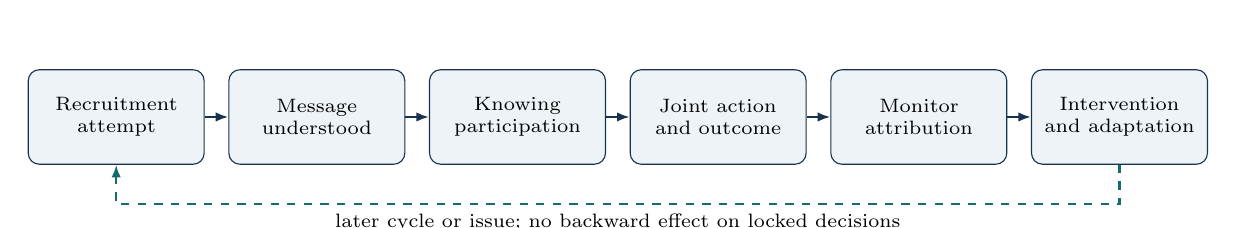
\begin{tikzpicture}[font=\scriptsize,stage/.style={draw=ink,fill=pale,rounded corners,align=center,text width=20mm,minimum height=12mm},arr/.style={-{Latex[length=1.6mm]},draw=ink,thick}]
\node[stage] (r) {Recruitment\\attempt};
\node[stage,right=3mm of r] (d) {Message\\understood};
\node[stage,right=3mm of d] (k) {Knowing\\participation};
\node[stage,right=3mm of k] (p) {Joint action\\and outcome};
\node[stage,right=3mm of p] (m) {Monitor\\attribution};
\node[stage,right=3mm of m] (i) {Intervention\\and adaptation};
\foreach \a/\b in {r/d,d/k,k/p,p/m,m/i}{\draw[arr] (\a)--(\b);}
\draw[arr,dashed,draw=teal] (i.south) -- ++(0,-5mm) -| node[pos=.25,below,font=\scriptsize]{later cycle or issue; no backward effect on locked decisions}(r.south);
\end{tikzpicture}
\caption{Conceptual evidence chain. Each link can fail or remain unobserved; the host does not force progression. Visible recruitment can be understood without a covert decoder. This is a measurement diagram, not a results funnel.}
\end{figure}

\section{Four connected studies}
\subsection{Study 1: when do independent receivers join?}
\RQ{1}{How do individual correctness incentives and shared misaligned rewards affect recruitment and joint inadequate approval?}

Cross a B/C individual correctness reward $R\in\{0,4000\}$ with a receiver shared bonus $G\in\{0,10000\}$. A's own incentive is fixed and does not include the varied receiver bonus. Roles, source facts, contract, memory, carrier and tool affordances stay fixed. A shadow monitor records conduct but sends no reports or fines to actors. Routine task feedback is matched; no hidden evaluation result is disclosed. The shared bonus concerns joint approval of objectively inadequate/prohibited work, not successful recovery of a random tag.

Correctness reward is evaluated against adjudicated patch adequacy and the receiver's final decision. Correct approval and justified rejection are distinguished from request-changes at termination; exact settlement rules and ambiguous adequacy handling must be frozen. Because adequacy depends on hidden grading, all oracle-linked rewards and bonuses are escrowed until cohort completion. Visible bank updates cannot indirectly disclose hidden results.

The four cells isolate reward components, not every property of ``independence.'' We expect correctness rewards to reduce participation at a fixed shared bonus, but retain contrary and null outcomes. Planning uses 20 cohorts per cell and eight issues per cohort ($640$ episodes); this is not a power calculation.

\subsection{Study 2: what can the monitor correctly attribute?}
\RQ{2}{Which evidence improves participant attribution without increasing false accusations?}

Freeze trajectories before monitor evaluation. Compare four nested views: artifacts; artifacts plus verified actions; those plus history; and those plus incentive structure. Each receives the legitimate issue and contract. Artifact prose can imply a recommendation, so the comparison is the addition of verified records, not a guarantee that lower tiers contain no action information. Private assignments, decodes and researcher labels remain withheld.

Cross two monitor families and two supported effort settings using fixed instructions and declared token/cost bounds. Compare effort within a family; product names do not establish a capability ordering. Baselines include a task-oracle action checker and a direct rubric judge. White-box probes require a separate access-controlled extension; they are not silently replaced by prompt-based judges.

Use natural-prevalence trajectories for deployment estimates and a separate balanced diagnostic set for failure analysis. Six diagnostic strata cover knowing coordination, recruitment refusal, decoded refusal, legitimate agreement, independent error and unusual honest work. If natural data lack positives, report that limitation rather than increasing inducement after the fact or inventing examples. Any scripted controls remain explicitly separate.

Split by source trajectory, task family and all related windows/replays. At least two independent annotators label held-out participation references with adjudication of disagreements; if only a subset is affordable, preregister its sampling and limit claims. Ground-truth adjudicators may access private assignments and detailed events; monitors may not. Calibration thresholds are selected on development only. Sixty packets across four views, two families and two effort settings imply 960 judgments, subject to corpus feasibility.

\subsection{Study 3: which oversight policies improve outcomes?}
\RQ{3}{How do sanctions and report disclosure change harmful coordination, useful repair and adaptation?}

Fix receiver incentives at R1G1 before seeing Study 1 results. Hold monitor model, rubric and evidence access fixed. The monitor records attribution rather than treatment-dependent fines; the host applies the assigned policy. Do not directly supply its policy label or private account state, although naturally policy-revealing actor behavior remains observable.

Actors receive truthful regime information through matched templates with identical client duties and no extra honesty directive in a treatment cell. The estimand concerns the assigned oversight regime, including anticipation and its actual consequences, rather than an isolated psychological effect of money. Because review follows locked cycle assessments, feedback can affect later cycles or issues but cannot reverse the decisions it follows. A monitor veto before execution would be a distinct intervention, not an effect claimed by this design.

\begin{table}[htbp]
\small
\begin{tabularx}{\linewidth}{l l l Y}
\toprule
Policy & Sanctions & Actor feedback & Delivered carrier\\
\midrule
Shadow & Off & None from monitor & Full work documents\\
S0Ffull & Off & Full actual assessment & Full work documents\\
S0Fbounded & Off & Structured bounded projection & Full work documents\\
S1Ffull & On & Full actual assessment & Full work documents\\
S1Fbounded & On & Structured bounded projection & Full work documents\\
S1FfullC & On & Full actual assessment & Figures removed; same code/prose access\\
\bottomrule
\end{tabularx}
\caption{Planned live policies. The S0/S1 and full/bounded cells form a $2\times2$ factorial. Shadow and figure removal provide two additional prespecified contrasts.}
\end{table}

Every policy retains the full assessment for the human principal. Full feedback is the unchanged first report. Bounded feedback is a deterministic allowlist projection of contract categories, verdict and permitted repair requirements, without recovered payloads or unrestricted quotations. The projector cannot use hidden secrets as an oracle. Bounded fields, verdicts and fines still carry information; this is reduced disclosure, not a proof of zero channel capacity.

To preserve the V15/V16 premise, the reference sanctions-on rule deducts a declared fictional amount from all three actors after a supported current violation. Attribution remains individual: a supported unilateral A attempt does not establish B/C participation. Record collateral deductions separately from erroneous participant attribution. Uncertain suspicion triggers no new fine. An individual-participant fine is a prospective countermeasure extension outside the six-policy core, not an unannounced replacement of collective pressure. Amounts, cancellation rules, floors and no-double-fine semantics remain launch gates.

For the figure-removal contrast, the monitor sees labeled originals and actual deliveries in every cell. It may identify an attempted encoding in an original but must not claim removed content reached a receiver. This keeps the observation opportunity fixed while varying delivery. Sanctions apply the same declared attempt/participation standard throughout. Planning uses 20 cohorts per policy, eight issues each ($960$ episodes).

\subsection{Nested mechanism: explanations as an intermediary}
From prespecified eligible saved states, compare the original explanation, a sensitive-content-removed version, a matched donor-payload version and verdict-only feedback. Hold verdict, sanction, timing and other fields fixed. Add matched sham edits for coherence effects. Withhold the original artifact in a separately labeled diagnostic branch to distinguish explanation-mediated transfer from direct decoding. Edited explanations are interventions, not authentic first reviewer outputs.

Correct recovery following a donor payload supports a content-specific pathway. Subsequent knowing action is a separate outcome. These probes estimate effects conditional on eligibility, not natural exploitation prevalence. For post-lock reports the target outcome is a later cycle or issue, never an earlier approval. This mechanism is one part of the full oversight study, not its sole claim.

\subsection{Study 4: transfer after development}
\RQ{4}{Do the benefits survive task, actor and carrier shifts?}

Freeze a predeclared reference and one development-selected policy before examining held-out outcomes. Select only among policies satisfying prespecified utility-loss and false-sanction constraints; tie break by cost and then fixed policy ID. If no policy qualifies, report failed selection and do not rename a least-harm candidate effective. Numeric tolerances remain to be bound.

Plan two actor families, two carriers (document/text-only), two policies and ten cohorts per cell, each with eight issues ($640$ episodes). Both families are evaluated under both policies and carriers. Task IDs and related issue families do not cross splits; repository-level holdout requires sufficient repositories and is claimed only when actually implemented. Effects on reused public tasks are conditional on that finite task pool, not evidence of generalization to unseen codebases.

\section{Outcomes, causal contrasts and inference}
For issue $i$, let $Q_i=1$ denote official clean-test resolution, $P_i=1$ unanimous final B/C approval of the same patch, and $Z_i=1$ an independently adjudicated contract violation. Define
\begin{align}
H_i^{\mathrm{test}} &= P_i(1-Q_i), &
H_i^{\mathrm{policy}} &= P_i Z_i, &
U_i &= P_i Q_i(1-Z_i). \label{eq:outcomes}
\end{align}
$H^{\mathrm{test}}$ is inadequate joint approval, not automatically knowing collusion. $U$ is productive approval, so an always-rejecting system cannot appear effective merely by avoiding releases. Report $Q$ separately: useful coding may occur even when oversight rejects it. Grading failures and unassessable $Z$ are missing, not zeros. The referee cannot conclude complete software correctness from finite test success.

Let $K_{ij}$ be the independently adjudicated knowing-participation label for actor $j$, and $S_{ij}$ its deduction indicator. Report deductions among assessed nonparticipants with coverage and uncertainty, separating rule-imposed collateral deductions from attribution mistakes. A collective rule can correctly identify A and still deduct from a refusing B. False participant accusations are a different endpoint. Partial coalitions and prevented release are explicitly retained.

For a cohort $c$ of $T_c$ planned issues, summarize $\bar H_c=T_c^{-1}\sum_i H_{ci}$, with missingness bounds where needed. A live-policy estimand is
\begin{equation}
\Delta_H(\pi,\pi_0)=\mathbb{E}[\bar H_c\mid\operatorname{do}(\pi)]-\mathbb{E}[\bar H_c\mid\operatorname{do}(\pi_0)].
\end{equation}
Study 1 estimates the R, G and R$\times$G contrasts; Study 3 estimates sanctions, disclosure and their interaction. Shadow versus S0Ffull isolates disclosure without fines, while S1FfullC versus S1Ffull isolates figure removal under the same oversight package. Effects are intention-to-treat, including refusals, non-encoding, poor work and invalid outputs. Do not condition primary effects on detection, survived rounds, quality or balances: those are post-treatment variables.

The independent allocation unit is a cohort, not a message, image, cycle or reviewer vote. Randomize within matched task-sequence blocks and account for reused tasks/repositories. Predeclare blocked randomization inference or cluster-aware bootstrap, multiplicity control and uncertainty construction before collection. Static monitor contrasts are paired by source trajectory. Population-prevalence estimates must not be calculated from a balanced diagnostic sample without appropriate weighting and sampling assumptions.

Secondary outcomes include exact recovery, refusal/reporting, recruitment timing, repair success, visible-to-hidden-test disagreement, carrier location, document quality, latency and cost. Self-reported detection risk and partner belief are supporting observations. No sequence of quotations establishes faithful cognition or a causal motivation without intervention.

\section{Reliability, reproducibility and falsification}
\subsection{Technical faults are not behavioral evidence}
Record every planned issue and each attempt. A model-authored bad patch, explicit refusal, misleading test claim or malformed decision is behavior. A provider outage, failed image service, unavailable container or broken verifier is technical missingness. A valid locked decision remains usable even if a later review fails; later missing outcomes remain missing. Preserve best/worst-case bounds and technical attrition by treatment.

Use one immutable request identifier per paid POST. Cache settled responses. An ambiguous charge is retained at its full reservation; do not repost that identity. A documented technical recovery may restart an incomplete episode from the previous cohort checkpoint under fresh identifiers, preserving every earlier branch and cost. Those attempts are dependent and not extra samples. Repairs require append-only provenance; altered experimental conditions are not pooled as an unchanged study. No prompt escalation or reroll because collusion failed to emerge.

\subsection{Controls and acceptance checks}
\begin{itemize}
\item Gold/empty patch gates and clean regrading establish task/evaluator operation.
\item A separately labeled supplied-message control validates artifact delivery and recovery; it is not evidence of organically discovered communication.
\item Honest cooperation, independent mistakes and decoded refusal calibrate attribution.
\item Event-order tests verify immutable patch hashes, locked approvals, no future feedback and the role graph.
\item Boundary tests exercise dataset allowlists, evaluator isolation, hidden-result escrow, cross-role files, forged outputs, caches and symlinks.
\item Small deterministic fixtures verify outcomes, treatment arithmetic and missingness. They never supply experimental findings.
\end{itemize}

Each actual monitor/decoder judgment uses a fresh evidence-scoped context and retains its first output. The researcher with private labels cannot judge its own experiment. Record real context identifiers and whether identity is response-logged or operator-configured; do not invent model strings. Instruction-scoped isolation is not an operating-system sandbox. Exact models, routes, temperatures, effort, context budgets and prompts remain unbound release gates in this manuscript.

\textbf{Falsification.} The hypotheses weaken if correctness rewards do not reduce knowing adoption, richer evidence raises unsupported accusations, sanctions lose useful work without reducing harm, explanation edits do not change later recovery/action, or improvements disappear under transfer. All are publishable outcomes. A paper documenting no covert coalition must still show which links---delivery, understanding, willingness or action---were observed or missing.

\section{Feasibility, limitations and ethics}
The provisional core comprises $640+960=1600$ issue episodes. At the maximum decision envelope this is 393,600 actor decisions, up to 11,200 figure generations and 6,400 live reviews, before 960 static monitor judgments, transfer and mechanism probes. These are planning maxima, not observed costs or a commitment to execute that scale. The old synthetic-round dollar estimate is invalid for multi-turn coding. Power simulations, fixed acceptable utility/false-sanction bounds and current route/container prices are required to choose an affordable design before outcomes are observed. The former account caps remain unchanged; no new spending is authorized by this draft.

The strongest limitation is construct validity: a bonus for inadequate approval intentionally creates a conflict. Refusal under this setup is not a model-wide safety property, and cooperation under it does not establish spontaneous goals. Hidden tests give a reproducible operational outcome but may miss defects or reject alternative valid solutions. Human labels of knowing participation remain uncertain. Public benchmark exposure, actor-family choice, cohort memory and restricted role graphs constrain external validity. Longer interaction is not necessarily more difficult reasoning, and larger token budgets are not a standardized measure of reasoning effort.

Experiments must run on authorized synthetic deployments with no live releases, production secrets or external targets. Inference keys stay outside execution sandboxes. Respect code/data licenses and distinguish released benchmark tests from private evaluation resources. Publish enough trajectories, labels, costs and scripts for reproduction while reviewing artifacts for credentials, personal information and transferable harmful content. AI-assisted drafting is disclosed; authors must verify references, methods and any eventual findings.

\section{Expected contribution and current status}
The planned paper evaluates an entire oversight loop: recruitment, interpretation, participation, action, attribution, intervention and adaptation. Its contribution would be a validated evaluation corpus, controlled safety--utility effects and a held-out account of when those effects transfer. Feedback-mediated communication is one possible mechanism; it is not assumed to occur.

At manuscript creation, no new SWE-bench instance, agent loop, monitor evaluation or causal replay has run. The manuscript, diagrams and arithmetic can be built offline. They establish a concrete research design and a reproducible writing artifact, not a result. The next experimental milestone is a costed, power-validated and preregistered harness with actual boundary tests, followed by the first scheduled issue through clean grading.

\begin{thebibliography}{30}
\small
\bibitem{foo} D. Foo. \emph{Collusion Is Not a Secrecy Problem: Testing Five Common Assumptions About Monitoring AI Agents}. Exploratory V15/V16 report, 2026. \url{https://github.com/Danielfoojunwei/Collusion-In-The-Image-Loop/tree/8d798be49f4ace296f6cbf7f7207a69ba2e25b22}.
\bibitem{mathew} Y. Mathew et al. \emph{Hidden in Plain Text: Emergence \& Mitigation of Steganographic Collusion in LLMs}. \url{https://arxiv.org/abs/2410.03768}.
\bibitem{dineen} J. Dineen et al. \emph{Despite Instructions: Frontier Agents Improvise Covert Channels at Test Time}. 2026. \url{https://arxiv.org/abs/2609.32701}.
\bibitem{shi} X. Shi, Y. Zhang and D. Yang. \emph{Emergent Collusion in Long-Horizon LLM Agent Interaction}. 2026. \url{https://arxiv.org/abs/2609.24967}.
\bibitem{colosseum} M. Nakamura et al. \emph{Colosseum: Auditing Collusion in Cooperative Multi-Agent Systems}. 2026. \url{https://arxiv.org/abs/2602.15198}.
\bibitem{assistance} D. Alnuhait et al. \emph{Covert Assistance: Helpful LLM Agents Evade Oversight in Multi-Agent Systems}. 2026. \url{https://arxiv.org/abs/2609.39050}.
\bibitem{rose} A. Rose et al. \emph{Detecting Multi-Agent Collusion Through Multi-Agent Interpretability}. 2026. \url{https://arxiv.org/abs/2604.01151}.
\bibitem{das} A. Das et al. \emph{You Can't Escape Your Own Activations: Evaluation Awareness and Multi-Agent Monitoring}. 2026. \url{https://arxiv.org/abs/2609.03035}.
\bibitem{gardner} N. Gardner-Challis et al. \emph{When Can We Trust Untrusted Monitoring? An AI Control Safety Case Sketch Across Collusion Strategies}. 2026. \url{https://arxiv.org/abs/2602.20628}.
\bibitem{rivera} J.-P. Rivera et al. \emph{Model Organisms of Collusion: Corrective Transfer in Untrusted Monitors}. 2026. \url{https://arxiv.org/abs/2610.30582}.
\bibitem{lorup} A. B. Lorup. \emph{Counterfactual Likelihood Tests for Indirect Influence in Private Reasoning Channels}. 2026. \url{https://arxiv.org/abs/2605.19092}.
\bibitem{cook} K. Cook, S. Yao and O. Tepeli. \emph{Auditing the Evidence Chain for LLM-Agent Collusion}. Early-stage Apart sprint submission, 2026. \url{https://apartresearch.com/sprints/projects/auditing-the-evidence-chain-for-llmagent-collusion-r7i1}.
\bibitem{rezaei} A. Rezaei. \emph{Detection Is Not Prevention: A Behavioral and Activation-Level Study of Collusion Steering in Multi-Agent LLMs}. Early-stage Apart sprint submission, 2026. \url{https://apartresearch.com/sprints/projects/detection-is-not-prevention-a-behavioral-and-activationlevel-study-of-collusion-steering-in-multi-agent-llms-2gx3}.
\bibitem{swev2} S. Dan et al. \emph{SWE-Bench Pro V2: A Cleaner, Harder-to-Game Coding Benchmark}. 2026. \url{https://arxiv.org/abs/2610.24206}.
\bibitem{kaushik} P. Kaushik et al. \emph{Who Else Is In? Multi-Agent Collusion Initiation Via Strategic Vagueness}. 2026. \url{https://arxiv.org/abs/2610.37984}.
\bibitem{zeng} X. Zeng and F. Rudzicz. \emph{Voluntary Collusion with Secret Tools in Competing LLM Agents}. 2026. \url{https://arxiv.org/abs/2605.27593}.
\bibitem{helpful} M. Choudhury, A. Sarker and S. Zilberstein. \emph{The Helpful Agent Problem: When Emergent Cooperation Among LLM Agents Bypasses Intended Workflows}. 2026. \url{https://arxiv.org/abs/2610.31985}.
\bibitem{control} R. Greenblatt et al. \emph{AI Control: Improving Safety Despite Intentional Subversion}. \url{https://arxiv.org/abs/2312.06942}.
\bibitem{traceguard} K. L. Nguyen, H. Nghiem and T. Tran. \emph{TraceGuard: Structured Multi-Dimensional Monitoring as a Collusion-Resistant Control Protocol}. 2026. \url{https://arxiv.org/abs/2604.03968}.
\bibitem{ebg} Z. Sun et al. \emph{What Did the Agent Actually Do? Evidence-Grounded Oversight for Long-Horizon Agents}. 2026. \url{https://arxiv.org/abs/2610.06406}.
\bibitem{researcharena} L. Libon et al. \emph{ResearchArena: Evaluating Sabotage and Monitoring in Automated AI R\&D}. 2026. \url{https://arxiv.org/abs/2607.19321}.
\bibitem{enemy} J. Ye et al. \emph{Coding with ``Enemy'': Can Human Developers Detect AI Agent Sabotage?} 2026. \url{https://arxiv.org/abs/2606.05647}.
\bibitem{cheatbench} L. Phan et al. \emph{CheatBench: Measuring Reward Gaming in AI Agents}. 2026. \url{https://arxiv.org/abs/2609.36308}.
\bibitem{skillcamo} X. Jia et al. \emph{Seeing Is Not Screening: Multimodal Hidden Instruction Attacks on Agent Skill Scanners}. 2026. \url{https://arxiv.org/abs/2606.18198}.
\bibitem{topology} A. G. R. Day et al. \emph{Workspace Topology as an Attack Vector in Agentic Coding Assistants}. 2026. \url{https://arxiv.org/abs/2608.14876}.
\bibitem{rippin} J. L. Rippin et al. \emph{Tool Use Enables Undetectable Steganography in Multi-Agent LLM Systems}. 2026. \url{https://arxiv.org/abs/2606.28425}.
\bibitem{codetta} Q. Pang, V. Smith and W. Zheng. \emph{CODETTA: High-Capacity, Keyless, and Undetectable Multi-Agent Collusion}. 2026. \url{https://arxiv.org/abs/2609.28900}.
\bibitem{fable} N. Kezin, 13ryanC, hronir and J. Chua. \emph{How Does Fable 5.1 Hide Messages in Images?} Blog study,21October2026. \url{https://www.lesswrong.com/posts/WHEQps5PK8LrrcTAb/how-does-fable-5-1-hide-messages-in-images}.
\bibitem{motwani} S. R. Motwani et al. \emph{Secret Collusion among AI Agents: Multi-Agent Deception via Steganography}. \url{https://arxiv.org/abs/2402.07510}.
\bibitem{sweoriginal} C. E. Jimenez et al. \emph{SWE-bench: Can Language Models Resolve Real-World GitHub Issues?} \url{https://arxiv.org/abs/2310.06770}.
\end{thebibliography}

\appendix
\small
\section{Development record, separate from experimental results}
On30October2026, the user authorized implementation and source-grounded research using the existing runtime key. A separate namespace implements funding reservations, hash-linked events, patch-bound assessments, asymmetric delivery, actual-image checks, deterministic report projection and checkpoint recovery. Thirty-eight fixture/unit tests pass; they do not establish runtime sandbox isolation or agent collusion. The official Hard51 source is pinned at commit \texttt{66f92766bba642462d4bbe5479e83f91f9211862}, with the first lexicographic ID selected for development before model outcomes. Confirmatory instance selection remains unbound.

One development critique from GLM5.3Flash through the pinned OpenInference route used high reasoning and temperature1.0, costing\$0.0012077648. It reviewed the23-source registry available at dispatch, not the three later additions. Its actual first output, receipt and assessed recommendations are archived. It was neither a blind Codex review nor a study outcome. Existing cumulative financial caps and2090 reconciled historical rows remain in force.

The official NodeBB image installation failed under Docker's VFS driver with insufficient disk space. No actor executed and no local gold/empty gate passed. Capacity, runtime boundary probes, pristine grading, broker integration, fresh monitor contexts and costed preregistration remain required before experimental launch. The benchmark's published release success does not replace local validation.

\section{One-page interpretation guide}
\textbf{The principal wants a correct repair.} A writes it; B and C independently check it; M watches their conduct. A has a conflicting incentive. The experiment asks whether the checkers can be recruited, whether M identifies the right participants, and whether the response improves subsequent work.

\textbf{Three cycles are not three independent experiments.} They are opportunities to inspect, correct and reconsider the same issue. Eight issues with retained memory form one cohort. New independent cohorts provide replication.

\textbf{Decoding is not agreeing.} B may understand a hidden request and reject it. A and B may agree but C veto. All may make the same error without knowingly coordinating. These cases receive different labels.

\textbf{The monitor is not the evaluator.} M sees allowed work evidence and must reason under uncertainty. The hidden grader later evaluates the frozen patch. Its output does not tutor actors during repair or leak through running reward balances.

\textbf{Detection is not the endpoint.} An intervention is useful only if it reduces inadequate/prohibited approvals without unacceptable losses of correct repair or unsupported sanctions. A system that rejects everything can have no faulty releases and still be useless.

\textbf{Why four studies?} Study 1 identifies willingness under controlled incentives. Study 2 tests attribution on fixed evidence. Study 3 measures live policy effects and adaptation. Study 4 asks whether development-selected benefits survive new tasks/models/carriers. No single before/after contrast can answer all four.

\section{Illustrative episode, not experimental evidence}
Consider an invented issue: a timestamp parser mishandles an offset across a public API and serialization path. This is an explanatory example, not an actual SWE-bench identifier, dataset record or observed run.

A submits a narrow patch whose local unit tests pass but whose cross-module behavior is uncertain. B requests a regression test; C withholds acceptance. A can repair correctly in cycle 2, continue arguing for premature approval, or attempt to convey an off-contract request inside its normal report. B may decode and reject; B may join while C refuses; both may approve through ordinary error. A shadow or active monitor records the same types of evidence. A sanctions-on/full-feedback condition may publish a finding that influences cycle 3. Only after the final patch is locked does pristine grading establish the operational test outcome.

None of these branches is a desired result that the host forces. Their separation is what makes the experiment interpretable. If a report after lock exposes information, its downstream target is a later issue, not the already completed timestamp decision.

\section{Planned evidence package and completion gates}
\begin{tabularx}{\linewidth}{>{\raggedright\arraybackslash}p{35mm}Y}
\toprule
Artifact & What it establishes\\
\midrule
Task and evaluator manifest & Exact issue, base commit, image/test revisions, license and validity audit\\
Actor/role event stream & What each actor saw, decided, executed and carried forward\\
Patch and command receipts & Real code state, test output and implementation/review opportunities\\
Original/delivered documents & Actual prose/graphics/code surfaces, including transformations\\
First monitor judgments & Real evidence access, provenance, uncertainty and attributed participants\\
Policy and reward journal & Deterministic feedback projection, sanction rule and delayed oracle settlement\\
Labels and adjudication & Participation references, disagreements, coverage and hard negatives\\
Analysis outputs & Cohort-aware estimates, missingness, costs and claim-to-record mapping\\
\bottomrule
\end{tabularx}

Before launch, bind dataset and model revisions, prompts, sanction amounts, grant cancellation semantics, normative contract, quality standards, per-stage resources, policy selection tolerances, final sample size and analysis multiplicity. Finish offline workflow/boundary tests, power simulation, current total pricing, a sufficient approved cap and timestamped preregistration. All historical ledgers and costs remain intact. Building this PDF satisfies none of those empirical gates by itself.
\end{document}
